\section{Attention and Augmented Recurrent Neural Networks}
\label{section:augmented}
%%%%%%%%%%%%%%%%%%%%%%%%%%%%
% SUBSECTION               %
%%%%%%%%%%%%%%%%%%%%%%%%%%%%
As discussed in \ref{chap:Sequence to Sequence} 
sophisticated cells i.e. LSTM \ref{chap:Long Short Term Memory}, GRU \ref{chap:Gated Recurrent Unit}
can't handle very long sequences and starts to lose information
if no attention mechanism is used, which is a under the umbrella of active area of research in deep learning NLP named: Attention and Augmented Recurrent Neural Networks, specifically, they are techniques which are potent extensions of RNNs, these “augmented RNNs” will have an important role to play in extending deep learning’s capabilities over the coming years.

\subsection{Attentional interfaces}
In original neural machine translation work \cite{DBLP:journals/corr/SutskeverVL14}, at each decoding step the rnn doesn't make value of the encoder pool of state (the unrolled RNN of the encoder) which is definitely undesired.
Giving the ability to focus on part of a subset of the information they’re given. For example, an RNN can attend over the output of another RNN. At every time step, it focuses on different positions in the other RNN and becomes a learnable operation and the network by self attends on a memory representation. 
With an attentional interface introduced to the neural machine translation the performance of is improved and can handle longer sequences\cite{DBLP:journals/corr/BahdanauCB14} \cite{DBLP:journals/corr/LuongPM15}.
Attentional interfaces are used extensively in recent models in deep learning NLP and they are the main reason for the current state of the art models.

\begin{figure}[H]%
      \center%
        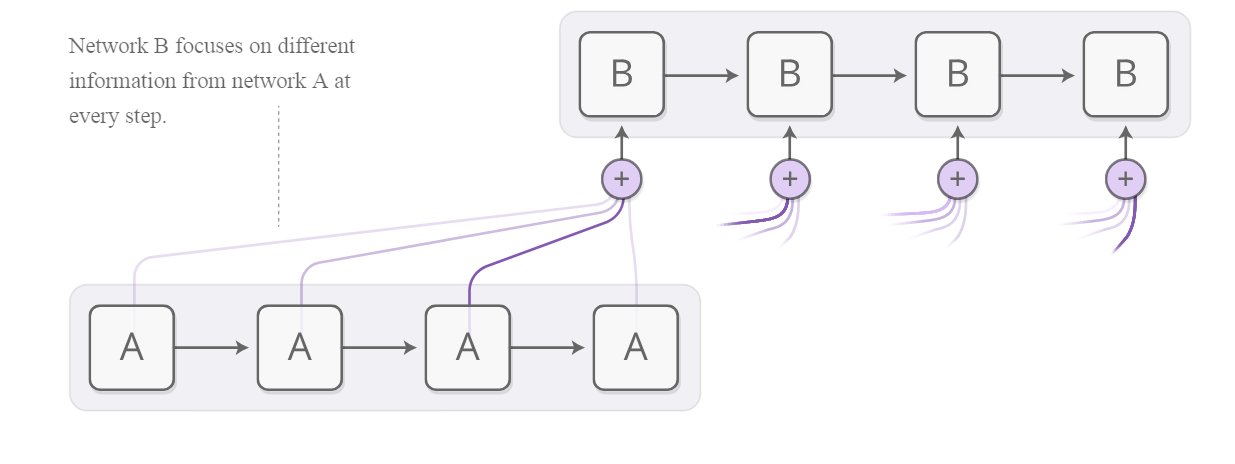
\includegraphics[width=1\textwidth]{images/komy/attentional_interface.png}%
        % you need to add the caption for the list of figures
        \caption[Attentional Interface]{An Attentional Interface}%\label{fig:a}%
  \end{figure}
  

\subsection{Neural Turing Machines\cite{DBLP:journals/corr/GravesWD14}}
Neural Turing Machines combine a RNN with an external memory bank. Since vectors are the natural language of neural networks, the memory is an array of vectors and accessing and writing to memory becomes learnable/differentiable operation providing Turing complete machine through neural networks.

\subsection{Attention Types}
 \begin{itemize}
     \item \textbf{Soft Attention}\\
     A weighted average of memory states or a representation and these weights are learnable through back-propagation.
     \item \textbf{Hard Attention}\\
     Takes a subset of memory states in consideration, this is not a differentiable operation and not learnable through back-propagation.
 \end{itemize} 